%----------------------------------------------------------------------------
\chapter{Sample application}
%----------------------------------------------------------------------------

This chapter presents the design and implementation of the sample application which will act as a case-study to showcase the features of the test framework and to serve as a basis for future enhancements. 


%----------------------------------------------------------------------------
\section{Design} \label{design}
%----------------------------------------------------------------------------

%----------------------------------------------------------------------------
\subsection{Requirements} \label{sample-app-requirements}
%----------------------------------------------------------------------------

%\begin{itemize}
%	\item objectives
%	\begin{itemize}
%		\item microservices architecture
%		\item containerization - facilitates easy deployment and scalability
%		\item have a system with different components based on state-fullness (stateful, stateless, )
%		\item have component(s) that can be scaled based on some application specific workload requirements (e.g. increased load on the system, fault tolerant redundancy) - stateless components can be scaled more easily
%		\item observable and collectible application specific metrics
%	\end{itemize}
%\end{itemize}

The design of the sample application was driven by several requirements to create a system that can be easily used for our purposes.

\paragraph{Kubernetes ready}The purpose of the thesis is to inspect dependability metrics in Kubernetes environments, this naturally means that the application should be able to run on a Kubernetes cluster.

\paragraph{Microservices architecture}As the application needs to be deployed and function in a Kubernetes-based environment, it was evident that a microservice architecture was the right choice for starting the design of the system. This notion implicitly means that there will be multiple, independent components that have to communicate with each other in order to create a whole system.

\paragraph{Scalability}In a real world application it is quite important to create systems that by design can handle different amount of workloads without any major impact on user experience. At the same time, an economic use of resources is also a significant requirement, so the system does not reserve too much resources and keeps them idle(\eg CPU, memory, storage, network bandwidth). That means the system should be able to dynamically change and fine tune its capacity and performance to satisfy both constraints. In addition, the application specific triggers for scaling should also be clearly defined.

\paragraph{Containerization}The ease of deployment and scalability is one of the cardinal goals of designing and maintaining a microservice application. Containerization provides the fundamentals for achieving this as all the dependencies and configuration needed for a component can be placed in a container. This leads to the conclusion that each component should be packaged and deployed into separate and independent containers.  In terms of scalability this form of packaging and deployment enables horizontal scaling, that means \eg during a bigger system usage, more instances of a given components should be started instead of increasing the resources of a single component instance.

\paragraph{Stateful and stateless components}The aim of the sample application is to attempt to provide a fair generalization of different kind of system components. A popular classification is deciding whether a component is stateful or stateless. This characteristic greatly affects how a given system is able to scale as stateless components are usually easier to manage in terms of scalability. To have the possibility of showcasing the scenario of scaling both types of components, there should be both stateful and stateless components in the case study system.

\paragraph{Observable application metrics}In order to be able to reason about the dependability and performance of the system, different kind of numerical metrics should be available to evaluate. This poses the requirement to create a system that can be easily monitored. The 
components should provide an interface that other tools can use to collect metrics describing both application specific behavior and the state of underlying layers (\eg CPU usage, memory usage, network communication).


%----------------------------------------------------------------------------
\subsection{Architecture}
%----------------------------------------------------------------------------

Although the aim of the sample application is to attempt to provide a generalized system to fit many use-cases without limiting possibilities, when it comes to architectural design, it is indispensable to create the structure of the system with a specific use-case in mind. But with a fairly common use case, the fundamental goal can be roughly preserved.

For this project, a master-worker architecture was chosen, where the master component receives input from clients and then assigns computational tasks to the workers based on the parameters. The computation should be resource heavy (\eg require much CPU time) and should last for an easily measurable time (minimum 30-40 seconds). This architecture allows to define scalable, and both stateful and stateless components. The abstract workflow of the use case is the following:

%TODO: activity diagram?

\begin{enumerate}
	\item \emph{Input submission} A client submits input parameters to the master component.
	\item \emph{Task distribution} The master component creates a task definition based on the input parameters and then forwards it to one of the worker components.
	\item \emph{Task execution} The worker components executes the received task and sends back the result to the master.
	\item \emph{Persisting results} The master persists the result of the completed task so it can be queried by clients.
\end{enumerate}

The designed architecture of the sample application can be seen in Figure \ref{fig:sample_app_arch}

\begin{figure}[h]
	\centering
	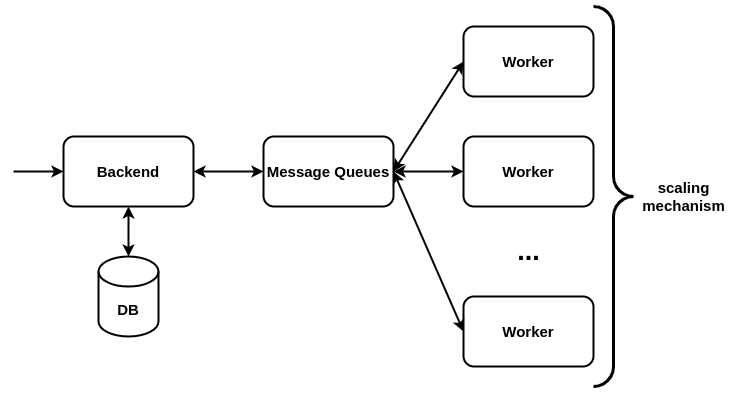
\includegraphics[width=130mm, keepaspectratio]{figures/sample_app_arch.png}
	\caption{Sample application architecture}
	\label{fig:sample_app_arch}
\end{figure}
%
%%----------------------------------------------------------------------------
%\subsection{Communication}
%%----------------------------------------------------------------------------
%
%Before commencing with the design of each component, it is important to specify how the components in the system will communicate with each other as this can affect their construction. Considering that the sample application tries to resemble implementations that are widely used in the industry, the components to be created in this project will expose REST API endpoints and will communicate over HTTP protocol. This provides the right degree of customizability on the component level while allowing loose-coupling on the system level. 


%\begin{itemize}
%	\item master-worker architecture
%	\item REST API interfaces
%	\item use-case
%	\begin{itemize}
%		\item submitting computation jobs
%		\item distributing jobs among worker nodes
%		\item persisting job results
%		\item querying job results
%	\end{itemize}
%	
%\end{itemize}


%----------------------------------------------------------------------------
\subsection{Components}
%----------------------------------------------------------------------------

In the following sections, each component and their responsibilities are presented.

%----------------------------------------------------------------------------
\subsubsection{Backend} \label{design-backend}
%----------------------------------------------------------------------------

%\begin{itemize}
%	\item provides a REST API interface for submitting new jobs and querying their result
%	\item forward submitted jobs to worker nodes
%	\item stores the result of finished jobs in a database
%	\item exposes a metrics endpoint for external monitoring solutions
%	\item exposes health endpoint that can be consumed to verify that the system works in a functionally correct way
%\end{itemize}
%
%responsibilites + API + health endpoint

The backend is responsible for handling task inputs from clients and creating task definitions based on them that it will forward to worker components. Upon receiving a task result from a worker, the backend persists the result in a database and makes it possible for clients to query it.

In order to be able to monitor the behavior and state of the backend component, it should be able to expose different kinds of metrics about itself. From an operations point of view it is quite important that each component have a so called health endpoint that can be used to tell if the given component is up and running. Clients and monitoring tools can consume this endpoint to make sure if a service is available. However, sometimes it is not enough information if a service is up or down. Consider one of the multiple cases when the backend is running, but suddenly the database connection is lost due to some failure. Although the backend is up but it cannot function correctly. This leads to the conclusion that when the health endpoint of the backend is consumed, the result should indicate if there are problems in any of the dependencies of the backend which can disrupt its correct functionality. This way the users and the maintainers of the service can be sure that the system can function correctly if the health endpoint returns without failure.

Summary of the required interfaces: \begin{itemize}
	\item Task input submission
	\item Task result query
	\item Health endpoint
\end{itemize}

%----------------------------------------------------------------------------
\subsubsection{Worker} \label{design-worker}
%----------------------------------------------------------------------------

%\begin{itemize}
%	\item provides a REST API interface to accept jobs from the backend to execute
%	\item exposes a metrics endpoint for external monitoring solutions
%	\item exposes health endpoint
%\end{itemize}
%
%responsibilites + API + health endpoint

The role of a worker instance is to listen for new task submissions from the backend and execute these tasks upon receiving them. Completed tasks should be sent back to the backend where the results will be saved in a persistent way.

Observability is essential here as well. The system needs to be able determine which worker instances are running and if there are idle ones that can accept new task submissions. If there is not any free worker, new instances should be deployed. If there are multiple idle workers but no task to execute, then the system should scale in, stopping a couple of idle worker instances. To achieve that, the worker component should be able to expose information about itself if it is up and if it is currently busy working on a task or not.


%----------------------------------------------------------------------------
\subsubsection{Message Queue} \label{design-message-queue}
%----------------------------------------------------------------------------

%\begin{itemize}
%	\item connects the backend with the worker nodes
%	\item as the number of worker nodes is dynamic, it would be not feasible for the backend to try to keep record of all the running workers
%	\item the backend sends the jobs to the workers via this message queue
%	\item the the workers also use this to send back the finished jobs (at the moment, we could skip the message queue on the way back, but this way we do not need much modification if there would be more than one backend in order to \eg be able to handle a bigger load)
%\end{itemize}

The goal of the message queue is to connect the backend and the worker instances. As the number of workers can dynamically change over time, it is not evident for the backend where to send new task assignments.

A possible solution could be that the backend somehow internally keeps track of the running worker instances but this would lead to much overhead both on the application logic level and on the network communication layer.

Instead, a third component - a message queue - is introduced to the system. As its name suggests, it is a queue which behaves like a \emph{First In First Out} buffer. The backend can push new task assignments to the queue without the need to know which worker instance will process it. On the other end of the queue the worker instances wait for new tasks in the queue and when one appears, one of the worker takes it from the queue and starts working on it. Notice that this method is also applicable for the other direction. To prepare for situations where there can be multiple backend components, the message queue can be used to by the workers to send back completed tasks to the backend service without knowing how many backend instances are actually in the system.

This pattern enforces loose coupling in the system and neither the backend nor the workers do not have to know about each other, they just need to know the message queue to produce and to consume new tasks. 

%----------------------------------------------------------------------------
\subsubsection{Database}
%----------------------------------------------------------------------------

%\begin{itemize}
%	\item stores the jobs with their result 
%	\item serves queries made by the backend component
%\end{itemize}

The database is responsible for storing the tasks in the system in a durable way. It provides an interface through which it is possible to execute CRUD operations on the task entities.

%----------------------------------------------------------------------------
\section{Implementation}
%----------------------------------------------------------------------------

This section describes the implementation details and their justification for each component in the sample application.

%\begin{itemize}
%	\item Introduce the general problem it solves (naive implementation of Fibonacci - this is implementation)
%	\item Docker
%\end{itemize}

%----------------------------------------------------------------------------
\subsection{The Task}
%----------------------------------------------------------------------------

The motivation for having a use-case that drives the architectural design was emphasized in the previous section (\ref{design}). The specific task that the system can execute is calculating the value of a given element in the Fibonacci sequence. The clients can send the backend which Fibonacci number to calculate as input. For example if the client sends the number 6 as input, a worker will execute a task which result will be 8.

At first glance, it seems to be an overly simple application, but one has to keep in mind, that the specific task that the worker components can execute is in fact can be anything. This simple computation was chosen, because it is easy to parameterize, the magnitude of the input correlates well with execution time and the implementation of the logic does not divert the focus from the main goals of the project.

%----------------------------------------------------------------------------
\subsection{Containerization}
%----------------------------------------------------------------------------

The section that describes the requirements of the sample application (\ref{sample-app-requirements}) states that containerization is crucial in order to create a scalable microservice application. There are several containerization technologies used in the industry, but perhaps the most popular is Docker \cite{Docker} which can be viewed as the de facto containerization technology adopted by the industry. Because of this, all the components in the system are packaged with Docker.


%----------------------------------------------------------------------------
\subsection{Backend}
%----------------------------------------------------------------------------

%\begin{itemize}
%	\item Spring Boot Java
%	\item introduce Job model
%	\item introduce REST API
%	\item db connection
%	\item introduce health check
%	\item introduce Message Queue integration
%	\item spring bootBuildImage - reference later in CI/CD pipeline
%\end{itemize}

The backend component is written in the Java programming language using the Spring Boot framework that facilitates easy creation of stand-alone, production grade Spring based applications that can be run with minimal configuration \cite{SpringBoot}.

%----------------------------------------------------------------------------
\subsubsection{Job model}
%----------------------------------------------------------------------------

% TODO class diagram?

To be able to easily manage tasks, model class named Job is defined that represents a single Fibonacci number computation. It is a common POJO (Plain Old Java Object) that stores the input and the result of a task along with an unique identifier. A summary the fields of the class can be seen in Figure \ref{fig:job_model}.

\begin{figure}[h]
	\centering
	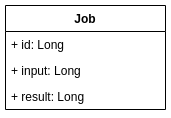
\includegraphics[width=40mm, keepaspectratio]{figures/job_class.png}
	\caption{Job class}
	\label{fig:job_model}
\end{figure}

%----------------------------------------------------------------------------
\subsubsection{Data persistence}
%----------------------------------------------------------------------------

When the backend component receives a task input from a client it creates a Job instance representing the task with an empty result and saves this object in the database. The reason of leaving the result field is evident as the task has not been executed by any of the workers and the backend does not know the result, but it is also quite practical to be able to tell at any point of the time which tasks have been completed and which have not. This feature will come handy when the test framework is used to measure the functional performance of the system.

The backend uses Spring Data JPA \cite{SpringDataJPA} to implement a data access layer without the need of having many lines of boilerplate code. To be able to store Job objects in the database, a couple of configurations should be made. The Job class needs to annotated with the \texttt{@Entity} annotation, indicating that this is a JPA entity so Spring Data JPA will know it must map this class in a table in the database. In order to be able to execute queries against the database in the program, a repository interface must be defined that Spring will use to generate the data accessing layer implementation with default CRUD operation. Lastly, the parameters of the database connection should be provided for the backend. This can be done in the \texttt{application.yaml}.

\vspace{0.5cm}
\begin{minipage}{\linewidth}
	\begin{lstlisting}[language=java, caption={\texttt{JobRepository} interface}, label={lst:JobRepository}]
		@Repository
		public interface JobRepository extends JpaRepository<Job, Long> {
			
			@Query("SELECT j FROM Job j WHERE j.result IS NULL")
			List<Job> findUnfinishedJobs();
			
			@Query("SELECT j FROM Job j WHERE j.result IS NOT NULL")
			List<Job> findFinishedJobs();
		}\end{lstlisting}
\end{minipage}

\vspace{0.5cm}
\begin{minipage}{\linewidth}
	\begin{lstlisting}[caption={Configuring the database connection}, label={lst:application-yaml-db}]
	# Database Properties
	database:
		host: ${MYSQL_DB_HOST:localhost}
		port: ${MYSQL_DB_PORT:3306}
		db: ${MYSQL_DB_DB_NAME:jobs}\end{lstlisting}
\end{minipage}

In \texttt{JobRepository} two additional methods are defined which will be later used to query \texttt{Job}s based on if they are completed or not.

%----------------------------------------------------------------------------
\subsubsection{Messaging}
%----------------------------------------------------------------------------

% TODO do we need more details?

As described in section \ref{design-message-queue} the backend uses a separate component acting as a message queue to forward new tasks to the worker components. This component (introduced later in section \ref{impl-message-queue}) implements the JMS API \cite{JMS} to handle messages between Java based applications.

This means that the backend should also use JMS to be able to send the tasks to the message queue. The implementation of this was inspired by the official Spring guide on handling messages with JMS \cite{JMSGuide}. The essential part is to configure a \texttt{JmsTemplate} that uses a connection to the message queue and using this object to send or receive messages. The actual implementation can be found under \texttt{messaging/activemq} package of the backend source code in the thesis repository \cite{ThesisRepo}.

%----------------------------------------------------------------------------
\subsubsection{Health check} \label{impl-backend-healthcheck}
%----------------------------------------------------------------------------

The importance of an mechanism that can determine if the backend is able to function correctly was mentioned in section \ref{design-backend}. As the system builds up from multiple components, checking if every part is working right consists of several steps. In the backend component, the health check includes four steps:

\begin{enumerate}
	\item \emph{Test database connection - }The backend test the connection to the database by attempting to save a test object. If it cannot be executed, the health check fails.
	\item \emph{Test worker availability - }The backend test the availability of the worker service by calling its health endpoint (described later in section \ref{impl-worker-interfaces}). If it returns with error, the the health check fails.
	\item \emph{Test message queue connection - }The backend sends a test message to the message queue which will be forwarded to one of the workers that will send back a reply. If the response is not received after a short amount of time, the health check fails.
	\item \emph{Test entire workflow with sample input - }Every 90 seconds the backend creates a dummy \texttt{Job} instance and sends it to the message queue and waits for response. Other non-test task execution reset the timer on this check. If there are not any successful task executions (dummy or real) in the last 90 seconds, the health check fails.
\end{enumerate}

%----------------------------------------------------------------------------
\subsubsection{Interfaces} \label{impl-backend-interfaces}
%----------------------------------------------------------------------------

The backend implements the interfaces described in section \ref{design-backend}.

\paragraph{Task input endpoint} This endpoint handles new task submission. Upon calling this endpoint the backend creates a \texttt{Job} instance with an empty result, saves it to the database and forwards it to the message queue.
\begin{itemize}
	\item \emph{Path - } \texttt{/api/v1/jobs}
	\item \emph{HTTP method - } \texttt{POST}
	\item \emph{Body - } a JSON object that has a single field named \texttt{input} with an integer value.
	\item \emph{Response - } a JSON object representing the created task (with empty result)
\end{itemize}

\paragraph{Task query endpoint} This endpoint can be used to retrieve all the tasks. Upon calling this endpoint the backend queries the database to get all the tasks stored there.
\begin{itemize}
	\item \emph{Path - } \texttt{/api/v1/jobs}
	\item \emph{HTTP method - } \texttt{GET}
	\item \emph{Body - } None
	\item \emph{Response - } a JSON array containing all the tasks stored in the database
\end{itemize}

\paragraph{Health endpoint} Upon calling this endpoint, the backend executes the health checks described in section \ref{impl-backend-healthcheck}.
\begin{itemize}
	\item \emph{Path - } \texttt{/api/v1/health}
	\item \emph{HTTP method - } \texttt{GET}
	\item \emph{Body - } None
	\item \emph{Response - } If any of the steps fail, the endpoint returns with a HTTP 500 response, otherwise with a HTTP 200 response.
\end{itemize}

%----------------------------------------------------------------------------
\subsection{Worker}
%----------------------------------------------------------------------------

%\begin{itemize}
%	\item Spring Boot Java
%	\item execution of tasks, implementation of fibonacci
%	\item introduce REST API
%	\item introduce Message Queue integration (same)
%	\item introduce health check
%	\item jobmodel (same)
%	\item spring bootBuildImage - reference later in CI/CD pipeline
%\end{itemize}

Similarly to the backend, the worker component is written in Java as well using the Spring Boot framework. It uses the same \texttt{Job} model as the backend an the implementation of the JMS messaging is also quite alike to that of the backend.

%----------------------------------------------------------------------------
\subsubsection{Task execution} \label{impl-worker-task-execution}
%----------------------------------------------------------------------------

The execution of tasks is handled by two classed in the worker component: \texttt{WorkerService} and \texttt{WorkerTask}. The \texttt{WorkerService} manages a thread pool that can run the computational tasks represented by \texttt{WorkerTask}. To make sure that a worker instance executes only one task at a time, the size of the thread pool is fixed at one thread. The \texttt{WorkerService} exposes the method \texttt{submitJob} that enables submitting a new \texttt{WorkerTask} which implements the \texttt{Runnable} interface. The \texttt{WorkerTask} stores a reference of the \texttt{Job} model, so it is aware of the parameters of the task. Inside its \texttt{run()} method, it calculates the given Fibonacci number and sends it back to the message queue.

The implementation of calculating a Fibonacci number can be seen below.

\vspace{0.5cm}
\begin{minipage}{\linewidth}
	\begin{lstlisting}[language=java, caption={Calculating Fibonacci numbers}, label={lst:fibonacci-method}]
	private long fibonacci(long n) {
		long result = 0L;
		if (n <= 2) {
			return n - 1;
		}
		result = fibonacci(n - 1) + fibonacci(n - 2);
		return result;
	}\end{lstlisting}
\end{minipage}

This implementation is not efficient as it does a lot of work repeatedly as it calculates the same values multiple times. However, increasing the performance of the worker is out of scope in this project. This algorithm is CPU heavy in its nature and the execution time can easily last for minutes with a large enough input, hence it satisfies the requirements defined in section \ref{design}.


%----------------------------------------------------------------------------
\subsubsection{Messaging}
%----------------------------------------------------------------------------

A notable difference is the configuration of the \texttt{PrefetchPolicy} of the message queue connection which tells the worker components to only consume one task from the queue at a time. This helps avoid scenarios where a worker instance takes out all the tasks from a queue and starts working on them sequentially leaving the rest of the workers without consumable task and causing them to remain idle in the system.

This setting can be configured for example in the \texttt{application.yaml} file where the message queue connection is specified.

\vspace{0.5cm}
\begin{minipage}{\linewidth}
	\begin{lstlisting}[caption={Configuring the message queue connection and modifying the default \texttt{PrefetchPolicy}}, label={lst:message-queue-connection}]
	# ActiveMQ
	activemq:
		broker:
			url: "tcp://${ACTIVEMQ_BROKER_HOST:localhost}:${ACTIVEMQ_BROKER_PORT:61616}?jms.prefetchPolicy.queuePrefetch=1"\end{lstlisting}
\end{minipage}

%----------------------------------------------------------------------------
\subsubsection{Health check}
%----------------------------------------------------------------------------

The worker component is in practice an independent unit in the system as long as it can connect to the message queue. This means that the implementation of the health check will not consist of so many steps as in the case of the backend component. In fact, simply returning without error during the health check can reliably indicate that the worker is able to function correctly.

%----------------------------------------------------------------------------
\subsubsection{Custom metrics} \label{impl-worker-custom-metrics}
%----------------------------------------------------------------------------

As the worker component can only process one task at a time by design, it is important that the worker should provide information about whether it is currently executing a test at a given point of time or not. This data can be used by the system to determine if should start more worker components in cases when there are tasks in the message queue waiting to be processed.

For this reason, the worker component exposes an application specific metric called \texttt{worker\_busy\_threads} that indicates how many threads are currently processing a task in a worker instance. This metric is published with the help of using a Micrometer \cite{Micrometer} library that facilitates exposing the metric in a Prometheus compatible format.

To achieve this, the custom metric is registered in the entrypoint class of the application, \texttt{WorkerApplication}.

\vspace{0.5cm}
\begin{minipage}{\linewidth}
	\begin{lstlisting}[language=java,caption={Registering a custom metric}]
	@Bean
	public MeterBinder busyThreads(WorkerService workerService) {
		return meterRegistry -> {
			Gauge.builder("worker.busy.threads", workerService::getBusyThreads).register(meterRegistry);
		};
	}\end{lstlisting}
\end{minipage}

The \texttt{WorkerService} has a method that returns how many threads are active at a given time. As the size of the threadpool is fixed at one, this method returns 0 or 1.

\vspace{0.5cm}
\begin{minipage}{\linewidth}
	\begin{lstlisting}[language=java,caption={Get the count of busy threads in the threadpool}]
	@Bean
	public int getBusyThreads() {
		return this.executor.getActiveCount();
	}\end{lstlisting}
\end{minipage}

Lastly, to configure Spring to expose the metrics, the desired endpoints should be enabled in the \texttt{application.yaml} file.

\vspace{0.5cm}
\begin{minipage}{\linewidth}
	\begin{lstlisting}[language=java,caption={Enabling Spring management endpoints}]
	management:
		endpoints:
			web:
				exposure:
					include: health,info,prometheus\end{lstlisting}
\end{minipage}

%----------------------------------------------------------------------------
\subsubsection{Interfaces} \label{impl-worker-interfaces}
%----------------------------------------------------------------------------

Based on the design described in Section \ref{design-worker} the worker exposes the following endpoints for the rest of the application.

\paragraph{Health} Upon calling this endpoint the worker returns with a HTTP 200 response. When the worker is down or encountered some critical error, this endpoint does not respond with anything so the caller will know that the worker is not functioning.
\begin{itemize}
	\item \emph{Path - } \texttt{/api/health}
	\item \emph{HTTP method - } \texttt{GET}
	\item \emph{Body - } None
	\item \emph{Response - } HTTP 200 response.
\end{itemize}

\paragraph{Metrics endpoint} This endpoint is provided by the Spring Boot Actuator that brings production-ready features to the application, for example various management endpoints.
\begin{itemize}
	\item \emph{Path - } \texttt{/actuator/prometheus}
	\item \emph{HTTP method - } \texttt{GET}
	\item \emph{Body - } None
	\item \emph{Response - } All the metrics exposed by the worker in a Prometheus compatible format.
\end{itemize}

%----------------------------------------------------------------------------
\subsection{Message Queue} \label{impl-message-queue}
%----------------------------------------------------------------------------

%\begin{itemize}
%	\item activemq
%	\item configuration? image?
%\end{itemize}

To accomplish the functionality of the message queue component introduced in Section \ref{design-message-queue} the Apache ActiveMQ \cite{ActiveMQ} product was used in the project. ActiveMQ is an open source, Java-based message protocol. Among the many protocol it implements, it supports forwarding JMS messages that the backend and the worker components use.

%----------------------------------------------------------------------------
\subsection{Database}
%----------------------------------------------------------------------------

%\begin{itemize}
%	\item mysql
%	\item configuration? image?
%\end{itemize}

The system uses MySQL \cite{MySQL} as the database which is an open source, relational database.

%----------------------------------------------------------------------------
\subsection{Deployment}
%----------------------------------------------------------------------------

%\begin{itemize}
%	\item aws eks
%	\item helm chart
%	\item K8s pod, depl, svc exapmle (one for each)
%	\item HPA definition, metrics server
%\end{itemize}

To be able to deploy the components, a running Kubernetes cluster is needed. Kubernetes can be set up manually on private machines but ususally the most feasible way to use Kubernetes is to exploit the managed Kubernetes service of a cloud provider. A managed Kubernetes means that the master nodes of the cluster (the control plane) are managed by a provider, taking off the operation burdens from users who have a simple way accessing the cluster.

There are many cloud providers that sell managed Kubernetes solution, in this project the product of Amazon Web Services is used called Elastic Kubernetes Service (EKS) \cite{EKS}.

All the above mentioned components are packaged with Docker and deployed to AWS EKS. In order to achieve that, various Kubernetes definitions are needed that are fairly similar in case of each component. In this section only the worker component related configurations and the definition of the Horizontal Pod Autoscaler are presented ot avoid unnecessary repetitions. However, all the definitions can be found in the thesis repository \cite{ThesisRepo} under \texttt{helm/kubedepend/templates}.

%----------------------------------------------------------------------------
\subsection{Helm chart}
%----------------------------------------------------------------------------

In order to facilitate easy deployment and configuration, a helm chart named \texttt{kubedepend} is created for the sample application that can be found in the thesis repository \cite{ThesisRepo} at \texttt{helm/kubedepend}.

Considering the nature of the project and the fact that most of the configuration settings do not change, the chart definition does not follow everywhere production grade best practices for sake of simplicity. That means that the majority of the configuration values are hard-coded into the helm templates instead of using template variables.

%----------------------------------------------------------------------------
\subsection{Kubernetes deployment}
%----------------------------------------------------------------------------

Deploying the worker component requires three type of Kubernetes definitions. First, a \texttt{ConfigMap} is used to store the configuration of the worker. A \texttt{Deployment} object is necessary to create a \texttt{Pod} that runs the worker in a container in a somewhat fault tolerant way using a \texttt{ReplicaSet}. Lastly, a \texttt{Service} is needed to create an unchanging address for the workers inside the cluster so other components can communicate with them.

%----------------------------------------------------------------------------
\subsubsection{Kubernetes ConfigMap}
%----------------------------------------------------------------------------

The necessary configurations for the worker component are defined using a \texttt{ConfigMap}. These values could also be specified directly in the \texttt{Deployment}, however, keeping them separately results in cleaner code.

In the example below, the parameters of the ActiveMQ connection and the queue names are defined for the worker.

\vspace{0.5cm}
\begin{minipage}{\linewidth}
	\begin{lstlisting}[caption={Worker \texttt{ConfigMap}}]
	apiVersion: v1
	kind: ConfigMap
	metadata:
	  name: worker-config
	  namespace: kubedepend
	data:
	  ACTIVEMQ_BROKER_HOST: kubedepend-activemq.kubedepend.svc.cluster.local
	  ACTIVEMQ_BROKER_PORT: "61616"
	  ACTIVEMQ_WORKER_QUEUE: jobWorkerQueue
	  ACTIVEMQ_BACKEND_QUEUE: jobBackendQueue\end{lstlisting}
\end{minipage}


%----------------------------------------------------------------------------
\subsubsection{Kubernetes Deployment}
%----------------------------------------------------------------------------

The worker \texttt{Deployment} declares how the cluster will control running the worker components. Several configuration parameters are set that can be seen in the following example.

\vspace{0.5cm}
\begin{minipage}{\linewidth}
	\begin{lstlisting}[caption={Worker \texttt{Deployment}}]
	apiVersion: apps/v1
	kind: Deployment
	metadata:
	  name: kubedepend-worker-depl
	  namespace: kubedepend
	spec:
	  selector:
	    matchLabels:
	      app: kubedepend-worker-app
	  replicas: 1
	  template:
	    metadata:
	      labels:
	        app: kubedepend-worker-app
	      annotations:
	        prometheus.io/scrape: "true"
	        prometheus.io/path: "/actuator/prometheus"
	        prometheus.io/port: "5000"
	    spec:
	      containers:
	      - name: kubedepend-worker
	        image: {{ .Values.worker.image.repository }}:{{ .Values.worker.image.tag }}
	        imagePullPolicy: Always
	        envFrom:
	        - configMapRef:
	          name: worker-config
	        resources:
	          requests:
	            memory: "512Mi"
	            cpu: "400m"
	          limits:
	            memory: "1024Mi"
	            cpu: "1500m"
	        ports:
	        - containerPort: 5000
	          name: worker-port\end{lstlisting}
\end{minipage}

The worker container that will run in a \texttt{Pod} is defined under the \texttt{spec} key. Here, the previously declared \texttt{ConfigMap} is referenced to use the values inside it as environment variables in the worker container. The \texttt{resources} section tells the cluster how much resource (CPU and memory) the container can use. This can help prevent the worker component from unnecessarily reserving too much resource, causing other components to starve. The \texttt{ports} section specifies the open port of the container and sets its name. This will be used when the \texttt{Service} object is defined for the worker. Under the \texttt{annotations} several monitoring related configurations are set to enable Prometheus scraping, further details in section \ref{test-impl-monitoring}.

The value of the \texttt{image} key is the only one that is not hard-coded. This is because every time the application is deployed, all the components get recompiled, rebuilt and packaged into a newly tagged docker image. Further details about the CI/CD pipeline in section \ref{cicd}.

%----------------------------------------------------------------------------
\subsubsection{Kubernetes Service}
%----------------------------------------------------------------------------

As the number of worker instances in the cluster can dynamically change, it is useful if there is a single, practically constant address that can be used to access the worker components. The Kubernetes \texttt{Service} can be used to define an abstraction that can be used to create a unique address in the cluster through which other components are able to access the individual worker components in a round robin way (see section \ref{k8s-service}).

\vspace{0.5cm}
\begin{minipage}{\linewidth}
	\begin{lstlisting}[caption={Worker \texttt{Service}}]
	apiVersion: v1
	kind: Service
	metadata:
	  name: kubedepend-worker
	  namespace: kubedepend
	  annotations:
	    prometheus.io/scrape: "true"
	    prometheus.io/path: "/actuator/prometheus"
	    prometheus.io/port: "5000"
	spec:
	  selector:
	    app: kubedepend-worker-app
	  ports:
	  - port: 5000
	    targetPort: worker-port\end{lstlisting}
\end{minipage}

In the example above the name of the port defined in the \texttt{Deployment} is used, so the \texttt{Service} is aware which port incoming requests should be forwarded to. Under the \texttt{annotations} several monitoring related configurations are set to enable Prometheus scraping, further details in section \ref{test-impl-monitoring}.


%----------------------------------------------------------------------------
\subsubsection{Horizontal Pod Autoscaler} \label{impl-hpa}
%----------------------------------------------------------------------------

% TODO HPA target instance calculation algorithm

The scaling of the worker component is managed by a Horizontal Pod Autoscaler. This object scales the target component (the worker \texttt{Deployment}) based on a custom metric. Whenever the value of the metric differs from the target value (defined under \texttt{spec.metrics.[0].target.value = 1}) the HPA will start a new or stop a worker component to restore the metric value to the target value.

The metric value is based on the number of messages waiting in the message queue, the number of currently busy workers executing tasks and the total number of worker instances. To prepare for frequent task input submissions, a hot spare worker instance is always present. The metric is calculated with the following equation:

\[
	\texttt{needed\_worker\_ratio} = \frac{1 + \#\ of\ messages\ in\ queue + \#\ of\ busy\ worker\ instances}{\#\ of\ worker\ instances}
\]

\vspace{0.5cm}
\begin{minipage}{\linewidth}
	\begin{lstlisting}[caption={Worker \texttt{Horizontal Pod Autoscaler}}]
	apiVersion: autoscaling/v2beta2
	kind: HorizontalPodAutoscaler
	metadata:
	  name: worker-hpa
	  namespace: kubedepend
	spec:
	  scaleTargetRef:
	    apiVersion: apps/v1
	    kind: Deployment
	    name: kubedepend-worker-depl
	  minReplicas: 1
	  maxReplicas: 10
      metrics:
      - type: Object
	    object:
	      metric:
            name: {{ .Values.hpa.metricName }}
          describedObject:
            apiVersion: /v1
            kind: Namespace
            name: kubedepend
          target:
            type: Value
            value: "1"
      behavior:
        scaleDown:
        stabilizationWindowSeconds: 30 # default is 300\end{lstlisting}
\end{minipage}











